% =============================================================================
\section{Flights with memory}\label{sec:model}

\begin{figure*}[t]
\centering
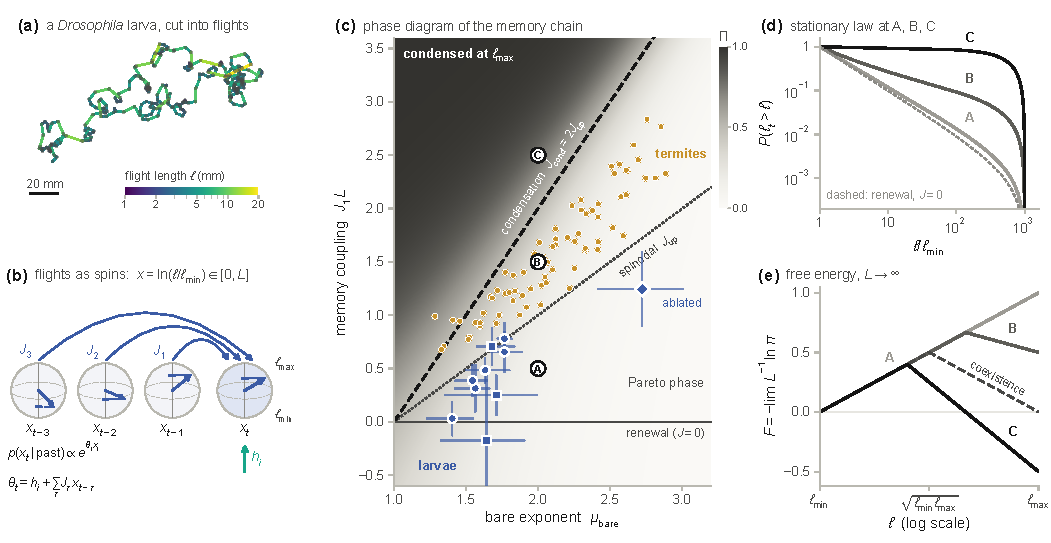
\includegraphics[width=\textwidth]{figs/fig1_overview.pdf}
\caption{From a track to a chain of spins. (a)~One hour of a \emph{Drosophila} larva (shi/+, 33\,$^\circ$C) crawling on plain agar: the flights (black segments, dots at the turns) cut out of the recorded track (grey). (b)~In the variable $x=\ln(\ell/\lmin)\in[0,L]$ a flight is the vertical projection of a classical spin on a sphere whose poles are the cutoffs $\lmin$ and $\lmax$; shown are four consecutive flights of the larva in (a). The next flight $x_t$ feels a field $h_i$, specific to the walker, and the previous flights through the couplings $J_\tau$, Eq.~\eqref{eq:causal}. (c)~Phase diagram of the chain with one lag, in the plane of the bare exponent $\mub=1-h$ and of the coupling $J_1L$. Shading: fraction $\Pi$ of flights longer than $\sqrt{\lmin\lmax}$ for $\lmax/\lmin=10^2$. Dotted, the spinodal $J=\Jup$; dashed, the self-dual condensation line $J=\Jcond=2\Jup$, Eq.~\eqref{eq:thresholds}. Indigo: larval conditions (median and interquartile range of $\mub$ over larvae, $\pm2$ s.e.\ of $J_1L$; circles, controls; squares, neurons silenced; diamond, brain lobes and sensory neurons ablated); ochre: 75 termite workers (Sec.~\ref{sec:data}). (d)~Stationary distribution of flight lengths at the states A, B and C marked in (c), for $\lmax/\lmin=10^3$; dashed, the renewal walk with the same $\mub$. (e)~Free energy $F(u)=-\lim_{L\to\infty}L^{-1}\ln\pi$ along $u=\ln(\ell/\lmin)/L$, Eq.~\eqref{eq:freeenergy}. It is piecewise linear because the stationary weight is a product of exponentials in $x$. In A the only minimum is at $\lmin$; in B a second, higher minimum at $\lmax$ makes runs of long flights metastable; on the dashed coexistence line the two minima are degenerate; in C the flights condense at $\lmax$.}
\label{fig:overview}
\end{figure*}

\subsection{One flight}\label{sec:single}

A flight length has no natural unit, so we measure it on a logarithmic scale. Every data set also comes with two bounds: a shortest flight $\lmin$, set by the resolution of the measurement, and a longest one $\lmax$, set by the walker, by the arena or by the duration of the recording. We keep both from the start and work with
\begin{equation}
x=\ln\frac{\ell}{\lmin}\in[0,L],\qquad L=\ln\frac{\lmax}{\lmin},
\label{eq:x}
\end{equation}
so that $L$ counts the $e$-folds spanned by the flights, between 3 and 6 for the walkers of Sec.~\ref{sec:data}. The measure $dx=d\ell/\ell$ is the only one that a change of units leaves invariant, up to a shift of $x$. Maximizing the entropy $S[p]=-\int_0^Ldx\,p(x)\ln p(x)$ at fixed $\langle x\rangle$ gives
\begin{equation}
p(x)=\frac{e^{\theta x}}{Z(\theta)},\qquad Z(\theta)=\frac{e^{\theta L}-1}{\theta},
\label{eq:single}
\end{equation}
which is a power law $p(\ell)\propto\ell^{-\mu}$ truncated to $[\lmin,\lmax]$, with $\mu=1-\theta$~\cite{Montroll1983}. (A MaxEnt law of flight lengths is thus a Pareto law; a L\'evy-stable law describes instead the sum of many flights.)

For a single flight, $\lmax$ is a convenience. On the half-line $x\ge0$, Eq.~\eqref{eq:single} is a normalized law whenever $\theta<0$, that is, $\mu>1$, and one may let $\lmax\to\infty$. The cutoff does make room for the opposite case: on $[0,L]$ any $\theta$ is allowed, and $\theta>0$ describes a walker whose flights pile up near $\lmax$. Section~\ref{sec:path} shows that, once flights remember each other, this case cannot be avoided, and the cutoff becomes a necessity.

The mean and the variance of $x$ are
\begin{equation}
\begin{aligned}
\langle x\rangle&=\Lambda(\theta)\equiv\frac L2\Big[1+\Lang\Big(\frac{\theta L}2\Big)\Big],\\
\mathrm{Var}\,x&=\Lambda'(\theta)=\frac{L^2}{4}\,\Lang'\Big(\frac{\theta L}2\Big),
\end{aligned}
\label{eq:langevin}
\end{equation}
where $\Lang(y)=\coth y-1/y$ is the Langevin function of paramagnetism [\figref{fig:theory}(a)]. Its appearance has a simple explanation. In the variable $u=2x/L-1\in[-1,1]$ the law~\eqref{eq:single} reads $p(u)\propto e^{bu}$ with $b=\theta L/2$. This is exactly the law of the vertical component $u=\cos\vartheta$ of a classical Heisenberg spin, a unit vector in three dimensions, in a field $b$: the area of a sphere between two heights is proportional to the distance between them (Archimedes' hat-box theorem), so $\cos\vartheta$ is uniform on $[-1,1]$ for a spin without field, and the Boltzmann factor $e^{b\cos\vartheta}$ tilts it as $e^{\theta x}$ tilts the flight. A flight is therefore a paramagnetic spin, which points to the south pole when the flight is close to $\lmin$ and to the north pole when it is close to $\lmax$ [\figref{fig:overview}(b)], and $\langle u\rangle=\Lang(b)$ is its magnetization. For the planar spins that describe directions of motion in Ref.~\cite{Agliari2024}, the Bessel ratio $I_1/I_0$ plays the same role. The susceptibility $\Lambda'$ is largest at $\theta=0$, where the histogram of $\ln\ell$ is flat and $\Lambda'(0)=L^2/12$; this number will set the critical point of the collective speed in Sec.~\ref{sec:meanfield}.

\subsection{A sequence of flights}\label{sec:path}

A walker produces flights $\mathbf x=(x_1,\dots,x_T)$ one after the other [\figref{fig:overview}(a)]. Following Ref.~\cite{Agliari2024}, in the spirit of maximum caliber~\cite{Presse2013}, we maximize the entropy of the whole sequence, $S[P]=-\int\mathcal Dx\,P[\mathbf x]\ln P[\mathbf x]$ with $\mathcal Dx=\prod_tdx_t$, at fixed mean of $x$ and fixed lagged correlations
\begin{equation}
C(\tau)=\frac1{T-K}\sum_{t=K+1}^T\langle x_tx_{t-\tau}\rangle,\qquad\tau=1,\dots,K .
\end{equation}
With Lagrange multipliers $h$ and $J_\tau$,
\begin{equation}
P[\mathbf x]=\frac1{Z_T}\exp\Big[\sum_tx_t\Big(h+\sum_{\tau=1}^KJ_\tau\,x_{t-\tau}\Big)\Big],
\label{eq:joint}
\end{equation}
the Boltzmann weight of a one-dimensional chain of continuous spins in time, in a field $h$ and with couplings $J_\tau$ of range $K$ [\figref{fig:overview}(b)]. For $K=0$ the flights are independent and identically distributed: this is the renewal L\'evy walk. A positive coupling means that long flights tend to follow long flights, a negative one that they alternate with short ones. With Gaussian instead of scale-free constraints the same construction gives Burg's maximum-entropy autoregression~\cite{Burg1975,CoverThomas}.

This is where the upper cutoff earns its place. Seen from flight $t$, the past acts as an effective field $h+\sum_\tau J_\tau x_{t-\tau}$. With $J_\tau>0$ this field grows with the length of the previous flights and, after long enough ones, becomes positive. On the half-line there is no normalizable law $e^{\theta x}$ with $\theta>0$, and the weight~\eqref{eq:joint} itself cannot be normalized. On $[0,L]$ every history yields a proper law, and every value of the parameters is allowed. What the cutoff costs is a scale: the largest change of field that one flight can produce on another is $J_\tau L$, and it is this product, not $J_\tau$ alone, that measures the strength of the memory (Sec.~\ref{sec:condensation}).

When several walkers are observed together, we give each walker $i$ its own field $h_i$. The fields absorb the differences between individuals, a quenched random field in the language of disordered systems, while the couplings, which describe the memory, are shared.

\subsection{The causal chain}\label{sec:causal}

The normalization $Z_T$ couples all the flights of Eq.~\eqref{eq:joint}, which makes its likelihood costly to evaluate. Agliari \emph{et al.} removed the difficulty with a mean-field step~\cite{Agliari2024}: in the weight of each spin they replaced the field generated by the past with the value it takes on the observed data, and normalized spin by spin, which makes the measure factorize in time. For one walker this step has an exact meaning. Each factor becomes the law of the next flight given the observed previous ones,
\begin{equation}
p(x_t\,|\,x_{t-1},\dots,x_{t-K})=\frac{e^{\theta_tx_t}}{Z(\theta_t)},\qquad
\theta_t=h+\sum_{\tau=1}^KJ_\tau\,x_{t-\tau},
\label{eq:causal}
\end{equation}
and their product is the probability of the observed sequence under a Markov chain of order $K$. This chain is a MaxEnt object in its own right: it maximizes the causal entropy $\sum_tH(x_t\,|\,x_{t-1},\dots,x_{t-K})$ under the same constraints~\cite{Ziebart2013}, and it is the model we use. At each turn the walker draws a truncated power law whose exponent, $\mu_t=1-\theta_t$, is set by its recent flights.

The log-likelihood
\begin{equation}
l(h,\bm J)=\sum_t\big[\theta_tx_t-\ln Z(\theta_t)\big]
\label{eq:loglik}
\end{equation}
is an elementary function of the parameters, and it is concave, because $\ln Z$ is convex and $\theta_t$ is linear in $(h,\bm J)$. Its maximum, when it exists, is unique. The stationarity conditions,
\begin{equation}
\sum_t\big[x_t-\Lambda(\theta_t)\big]=0,\qquad\sum_t\big[x_t-\Lambda(\theta_t)\big]\,x_{t-\tau}=0,
\label{eq:score}
\end{equation}
are the dynamic version of moment matching: the difference between each flight and its predicted mean must vanish on average and be uncorrelated with the past. The Fisher information,
\begin{equation}
\mathsf I=\sum_t\Lambda'(\theta_t)\,\bm z_t\bm z_t^{\mathsf T},\qquad \bm z_t=(1,x_{t-1},\dots,x_{t-K}),
\label{eq:fisher}
\end{equation}
gives the error bars. No Gaussian surrogate of the likelihood is needed: Eq.~\eqref{eq:loglik} is maximized as it is.

The path measure~\eqref{eq:joint} and the causal chain~\eqref{eq:causal} are different families with the same sufficient statistics. They agree to first order in $J$, after a shift of the field, and fitted to the same flights they return nearly the same couplings (Appendix~\ref{app:single}). In both, the selected depth is a Markov order~\cite{Ge2012}: $K^*=0$ is renewal, $K^*=1$ a Markov chain of flights, $K^*>1$ a longer memory. We call
\begin{equation}
\mub=1-h
\end{equation}
the bare exponent, the exponent of the next flight after a run of the shortest ones ($x_{t-\tau}=0$). With memory it differs from the exponent of the histogram of all flights (Sec.~\ref{sec:dressing}).

\begin{figure*}[t]
\centering
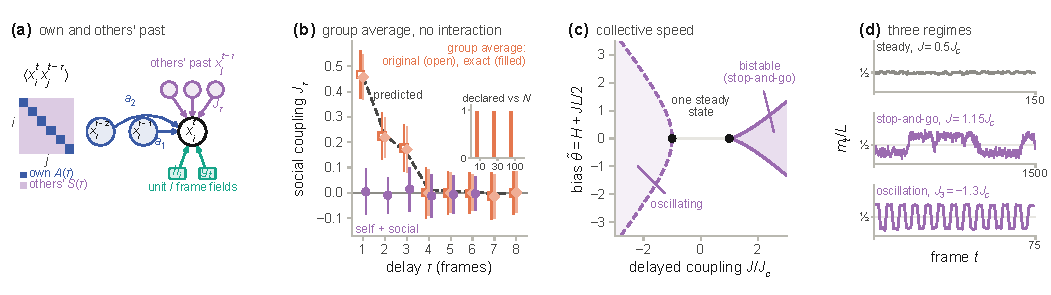
\includegraphics[width=\textwidth]{figs/fig2_many.pdf}
\caption{Many walkers. (a)~The lagged correlation between units has a diagonal part, each unit with its own past ($A$), and an off-diagonal part, each unit with the others' past ($S$); the group average mixes the two, Eq.~\eqref{eq:Rsplit}. The self\,+\,social model~\eqref{eq:selfsocial} gives each part its own couplings, $a_\tau$ and $J_\tau$, and adds a field for each unit, $h_i$, and for each frame, $g_t$. (b)~Synthetic units with own memory of depth 3 and no interaction ($N=30$, 40 replicates, mean $\pm$ s.d.): couplings returned by the group-average analysis in its original implementation (open squares) and with its exact likelihood (filled diamonds), against the prediction of Eq.~\eqref{eq:aggregation} (dashed); circles, social couplings of the self\,+\,social model. Inset: fraction of data sets in which a social coupling is declared, for $N=10$, 30 and 100. (c)~Mean-field phase diagram of the collective speed with one delayed coupling $J$, in units of $J_c=12/L^2$, and bias $\tilde\theta$: two stable states (shaded, solid boundary) for $J>J_c$, oscillations (dashed boundary) for $J<-J_c$; dots, the critical points. (d)~Group average on the symmetric line $\tilde\theta=0$: one steady state ($J=0.5J_c$, $N=200$), collective stop-and-go ($J=1.15J_c$, $N=40$), and oscillations of period 6 for a negative coupling at delay 3 ($N=200$). $L=\ln100$ throughout.}
\label{fig:many}
\end{figure*}

\subsection{Many walkers on a common clock}\label{sec:many}

In a group, the flights of different individuals start and end at different times, so ``the previous flight of the others'' is not defined. A group needs a common clock. We use frames $t$ of fixed duration and, for unit $i$, the log-displacement per frame, or log-speed, $x_i^t=\ln(\ell_i^t/\lmin)\in[0,L]$, with the same single-site law~\eqref{eq:single}.

Frames and flights are two different observables, and they answer different questions. On a frame clock a single flight spans many frames, so a walker's memory from one frame to the next mostly measures how long it keeps moving fast or slow; a renewal L\'evy walk observed in frames is strongly correlated, simply because its flights last. Whether a walker is a renewal process can only be asked of its flights, the events at which it chooses anew, and that is what we do for single walkers. Whether a walker responds to the others can only be asked on a common clock, and that is what we do for groups. The model is the same; only the index of time changes.

Transcribing Eq.~(A16) of Ref.~\cite{Agliari2024} from directions to log-speeds gives the path measure
\begin{equation}
P(\mathbf x)=\frac1Z\exp\Big[\sum_{t,i}x_i^t\Big(H+\frac1N\sum_{\tau=1}^{\tau_M}J_\tau\sum_jx_j^{t-\tau}\Big)\Big],
\label{eq:pre}
\end{equation}
which fixes the mean of $x$ and the lagged autocorrelation $R(\tau)=\langle m_tm_{t-\tau}\rangle$ of the group average $m_t=N^{-1}\sum_ix_i^t$. This autocorrelation contains two different things,
\begin{equation}
R(\tau)=\frac1NA(\tau)+\Big(1-\frac1N\Big)S(\tau),
\label{eq:Rsplit}
\end{equation}
where $A(\tau)$ is the mean lagged correlation of each unit with its own past and $S(\tau)$ that with the past of the others [\figref{fig:many}(a)]. In Eq.~\eqref{eq:pre} one multiplier $J_\tau$ accounts for both. Giving each its own multiplier, and each unit and each frame its own field, yields the self\,+\,social model,
\begin{equation}
\theta_i^t=h_i+g_t+\sum_{\tau=1}^{K_s}a_\tau\,x_i^{t-\tau}+\sum_{\tau=1}^{K_c}J_\tau\,s_i^{t-\tau},
\label{eq:selfsocial}
\end{equation}
with $p(x_i^t\,|\,\text{past})=e^{\theta_i^tx_i^t}/Z(\theta_i^t)$ and units independent of each other given the past of all. The self couplings $a_\tau$ are the memory of Sec.~\ref{sec:causal}. The social couplings $J_\tau$ act on $s_i^{t-\tau}$, the mean log-speed at frame $t-\tau$ of all other units (global coupling) or of the $k$ units nearest to $i$ (local coupling). The time fields $g_t$ absorb whatever affects all units at once. The model of Ref.~\cite{Agliari2024} is the special case $h_i=H$, $g_t=0$, $a_\tau=J_\tau/N$, $s=m$.

In Eq.~\eqref{eq:selfsocial} a unit's own past and the past of its neighbors enter in exactly the same way, as a field on its next step weighted by a coupling. Formally, the unit's own previous step is one more neighbor, the one that is always at distance zero: a memory is an interaction with one's own past, and an interaction is a memory of somebody else's. The two differ in what can produce them. Own memory can come from inertia, physiology or the persistence of a behavioral state; a coupling to the others' past requires that the unit perceives them, or that something drives both. They are kept in separate terms because the data offer them separately, in the diagonal and off-diagonal blocks of the lagged correlations of Fig.~\ref{fig:many}(a). For the same reason the single-walker model is not the trivial case $N=1$ of the collective one: it is the diagonal term that must be modeled before the off-diagonal one can be read.
